\section{TCGAbiolinks: An R/Bioconductor package to download and analyze data from GDC}

% Cancer is among the leading causes of death worldwide,
% and treatments for cancer range from clinical procedures
% such as surgery to complex combinations of drugs,
% surgery and chemoradiation (1). The Cancer Genome Atlas
% (TCGA), which began in 2006 with the aim of collecting
% and analyzing both clinical and molecular data
% on over 33 different tumor types by sampling across 500
% cases per tumor type, has to date generated the most
% comprehensive repository of human cancer molecular and
% clinical data (Figure 1A) (2). Tumors profiled by TCGA
% range from solid to hematological types, from mildly to
% severely aggressive in terms of survival and from benign
% to metastatic. For each cancer case, DNA, RNA and protein
% were extracted, and genomic, transcriptomic, epigenomic
% and (recently) proteomic (Figure 1B) profiling was
% then performed using a diverse set of ‘omics’ platforms,
% from custom microarrays to large-scale genomic sequencing.
% The TCGA consortium is organized into several
% working groups, each responsible for generating, collecting
% and coordinating data production (Biospecimen core
% resource and Data coordinating center) or analyzing the
% data (Genome data analysis center) (https://wiki.nci.nih.
% gov/display/TCGA/TCGA+Wiki+Home). \sigla{AWGs}{Analysis working groups} are formed by members of the scientific
% community to lead the data analysis for each tumor
% type (e.g. Breast or Kidney) and, more recently, for systemspecific
% cancers (e.g. central nervous system or reproductive
% system) or pan-cancer (all tumor types together) (2–6).
% AWG members download and analyze the currently publicly
% available data through the TCGA data portal (https://
% tcga-data.nci.nih.gov/tcga/). Members generally include experts
% in one or more data type (e.g. DNA methylation, expression,
% copy number or whole-genome sequencing) and
% experts in disease (generally oncologists specializing in each
% particular studied tumor). Using the collective knowledge
% gained by the experts in each platform and disease, a formal
% characterization and report is generated and published
% as a landmark TCGA marker (3,5–9).

% These findings have generated a wealth of advanced
% knowledge on the tumors reported and have led to the development
% of clinical prognostic and diagnostic biomarkers
% as well as redefinitions of prior classifications of tumors,
% as recently described in a study of lower-grade gliomas (3).
% The scientific cancer community has used TCGA data to
% advance their research and to provide even greater insight
% into these debilitating diseases, as evidenced by the growing
% number of citations of TCGA landmark papers (Figure
% 1C). In addition to advancing understanding of cancer,
% the TCGA data offer opportunities to develop novel statistical
% methodologies and create resources to integrate with
% other data consortia, such as the Roadmap (10) and Encode
% projects (11), as has been illustrated in a recent study
% by Yao et al. (12).

% Despite the wealth and accessibility of its data, TCGA
% presents several major challenges for bioinformaticians,
% clinicians and molecular biologists interested in harnessing
% TCGA data to further their own research (2,13,14).
% Among these researchers are data analysts who are interested
% in reproducing some of the major findings by the
% TCGA AWGs and incorporating novel methodologies into
% the preprocessing, processing and filtering steps, such as
% normalization, feature selection and downstream integrative
% analyses (13). However, the TCGA data and archives
% are constantly changing, either because of newly created
% data or because some data sets have been retracted by the
% families of the patients or the data were later discovered
% to be from the wrong tissue source or to be of low quality.
% To keep up with the dynamic and ever-changing structure
% of the TCGA data repository, the Data Coordination
% Center’s Web Service (DCCWS) was made available to access
% the TCGA database (https://wiki.nci.nih.gov/display/
% TCGA/TCGA+DCC+Web+Service+User’s+Guide). The
% DCCWS contains information about the centers, platforms,
% archives and other information relevant to the project. In
% addition, methodologies applied to analyze the TCGA data
% have mostly been presented in Sweave R documents or inhouse
% R scripts (15–17), thus making it challenging for
% many to harness the discoveries. Many studies, including
% TCGA marker papers, deposit supplementary tables with
% external websites, as PDF files, or Excel tables (https://tcgadata.nci.nih.gov/docs/publications/),
% thus making the effort
% to reproduce these findings or integrate them with one’s own
% data even more challenging.

% \begin{figure*}
% \centering
% %\includegraphics[width=.9\linewidth]{figures/case3_improved.pdf}
% 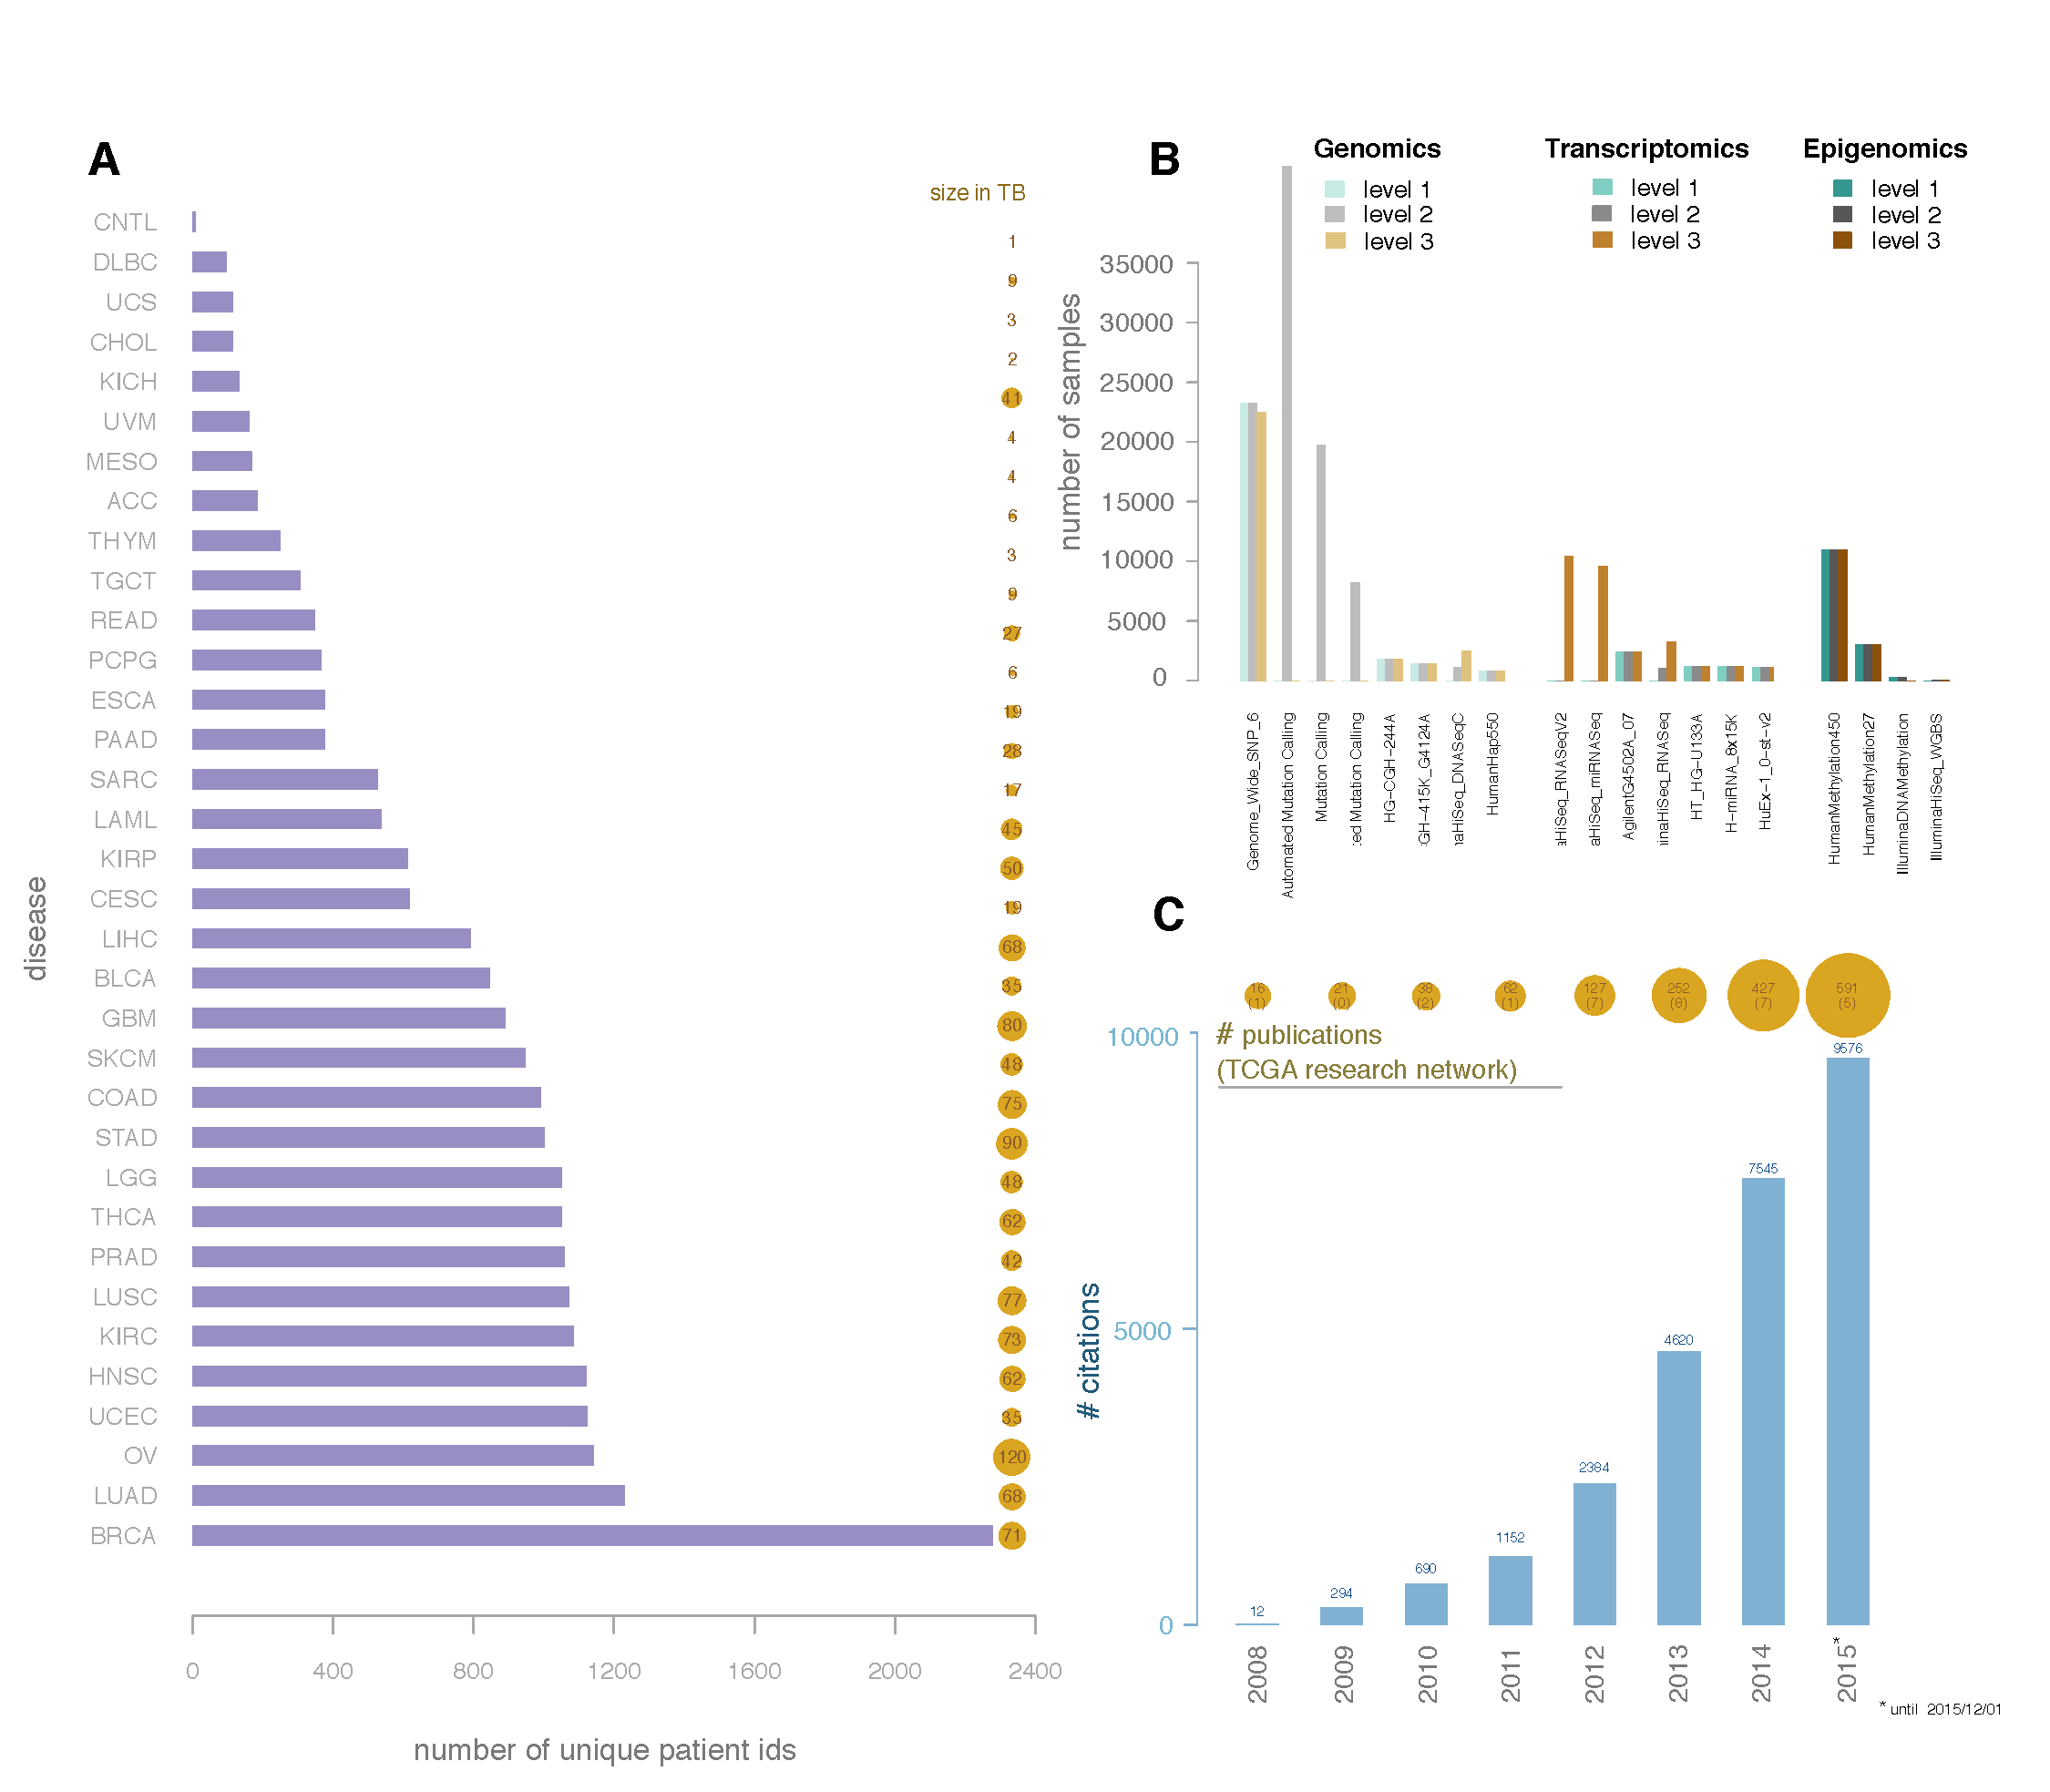
\includegraphics[width=1.0\linewidth]{images/figure1.pdf}
% \caption[TCGA data overview.]{TCGA data overview. \textbf{(A)} bars represent number of patients by disease; bubbles represent the available data size in TB by disease; \textbf{(B)} number of samples by platform and by level, grouped by type: genomic, transcriptomic and epigenomic. \textbf{(C)} Barplot: number of citations for TCGA papers. Bubble plot: number of TCGA papers, in parenthesis the number of papers published by the TCGA Research Network. Source: Scopus search for ’TCGA’, adding TCGA Research Network papers that were not found during this search. }
% \label{fig:tcgabiolinks1}
% \end{figure*}




The aim of TCGAbiolinks is four-fold: (i) to facilitate
data retrieval via GDC’s API; (ii) to prepare the data
using the appropriate preprocessing strategies; (iii) to provide
a means to conduct different standard analyses and
advanced integrative analyses and (iv) to allow the user to
easily reproduce earlier research results.
We introduce public methods
used in several marker papers to integrate DNA methylation
and gene expression data. In addition, our tool extracts
published molecular subtype information for each
TCGA sample within a tumor type (generally embedded in
supplementary tables, PDFs or external websites). Because
our tool was developed in the language of R specifically for integration within the Bioconductor project, we have provided most of the TCGA data objects as the Bioconductor specified
‘SummarizedExperiment’ class \cite{huber2015orchestrating}, thereby allowing easy integration with other data types and statistical
methods that are common in the Bioconductor repository.





\subsection{The TCGAbiolinks package}
TCGAbiolinks is an R package, which is licensed under
the General Public License (GPLv3), and is freely available
through the Bioconductor repository \cite{gentleman2004bioconductor}. By conforming to the strict guidelines for package submission to
Bioconductor, we were able to utilize and incorporate existing R/Bioconductor packages and statistics to assist in identifying differentially altered genomic regions defined by mutation, copy number, expression or DNA methylation; to reproduce previous TCGA marker studies; and to integrate data types both within TCGA and across other data types outside of TCGA. TCGAbiolinks consists of functions that can be grouped into three main levels: Data, Analysis and Visualization. More specifically, the package provides multiple methods for the analysis of individual experimental platforms (e.g. differential expression analysis or identifying
differentially methylated regions or copy number alterations) and methods for visualization (e.g. survival plots, volcano plots and starburst plots) to facilitate the development of complete analysis pipelines. In addition, TCGAbiolinks
offers in-depth integrative analysis of multiple platforms,
such as copy number and expression or expression
and DNA methylation, as demonstrated and applied in our
recent TCGA study of 1122 gliomas \cite{ceccarelli2016molecular}. These functions
can be used independently or in combination to provide the
user with fully comprehensible analysis pipelines applied to
TCGA data. A schematic overview of the package is presented
in Figure \ref{fig:tcgabiolinksfunctions}. The next subsections describe each of the three main levels (Data, Analysis and Visualization) below, highlighting the importance and utility of each associated function and sub-function.

\begin{figure*}
\centering
%\includegraphics[width=.9\linewidth]{figures/case3_improved.pdf}
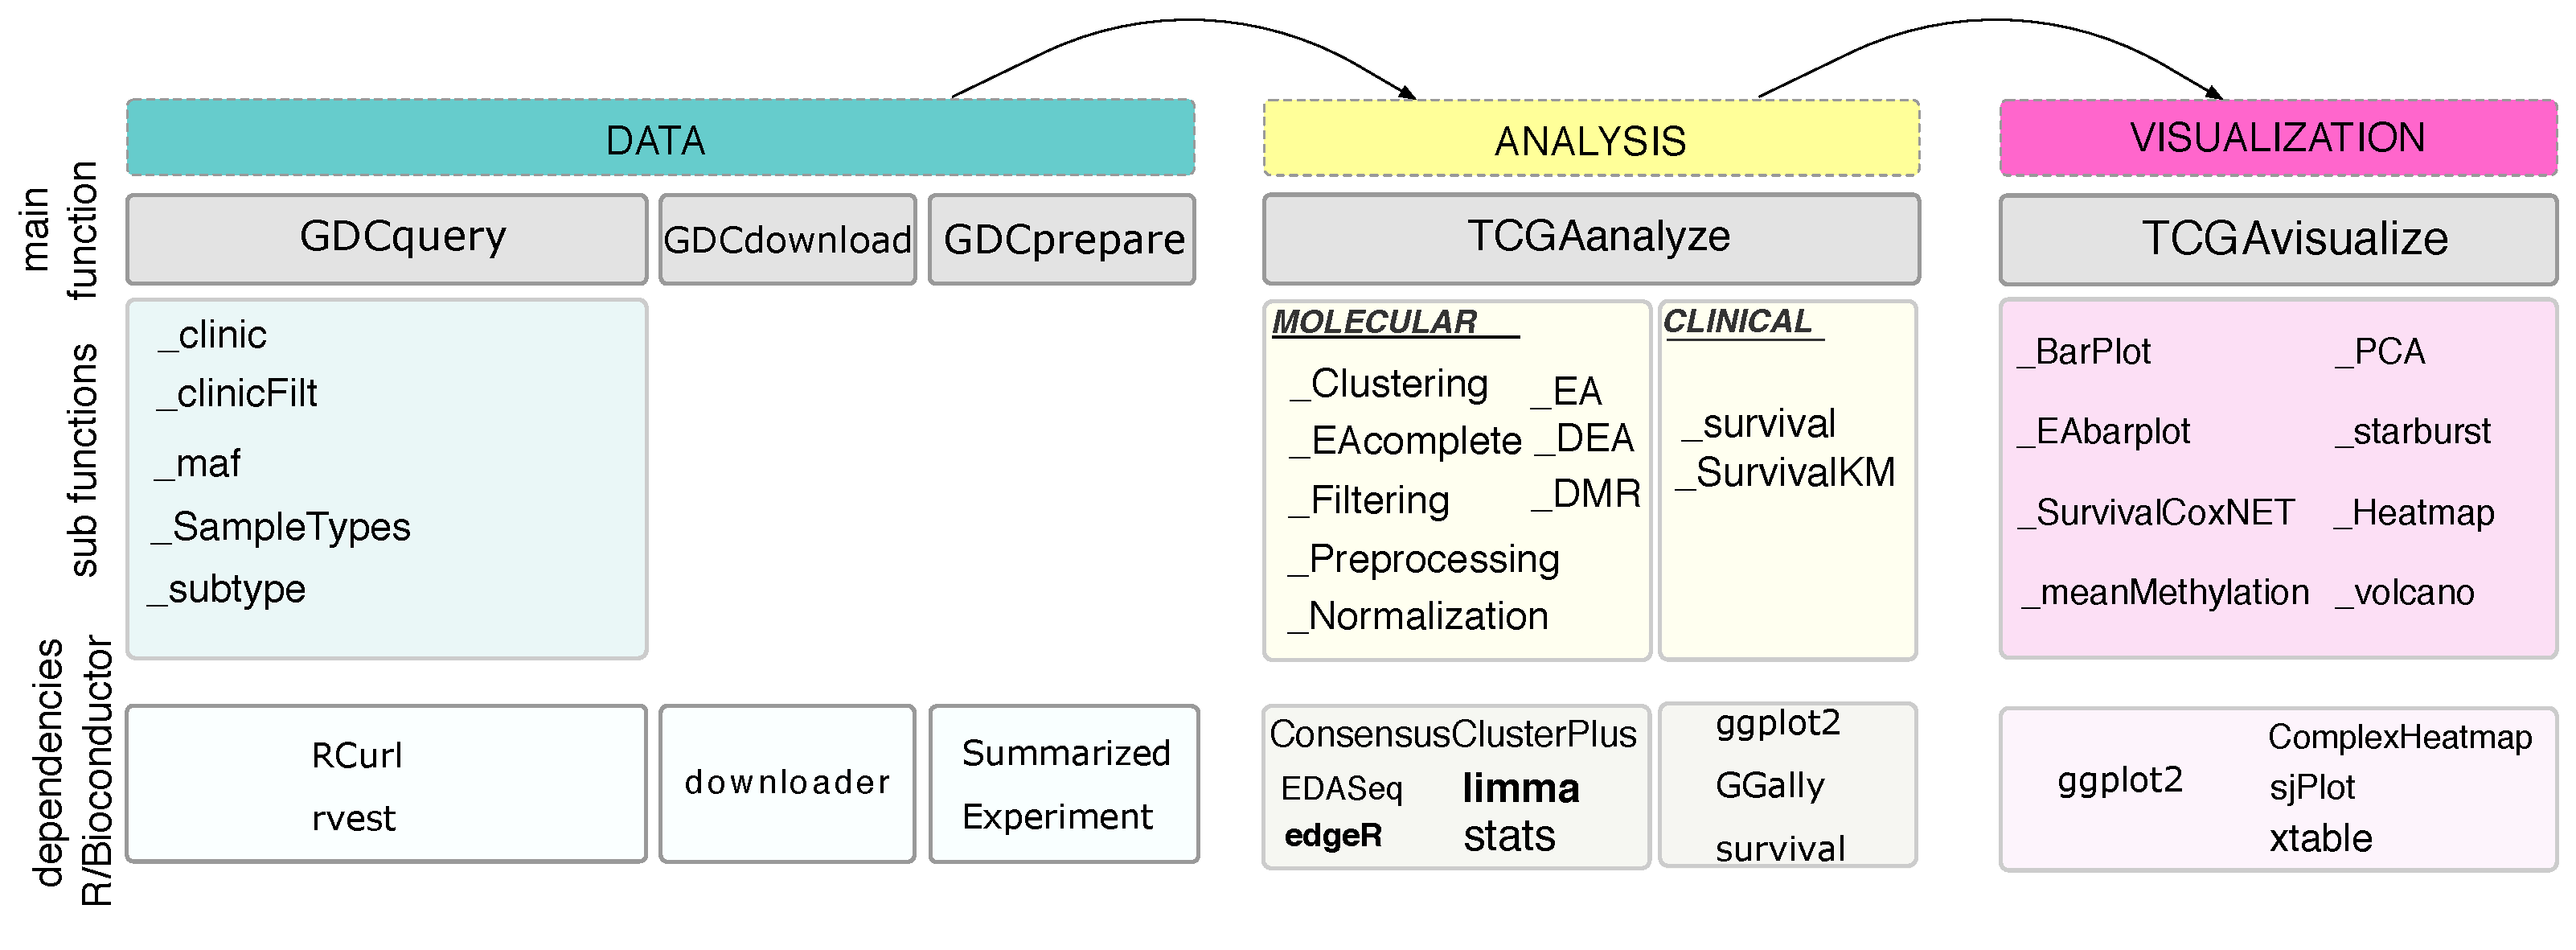
\includegraphics[width=1.0\linewidth]{images/figure1_new.pdf}


\caption[Overview of TCGAbiolinks functions.]{ Overview of TCGAbiolinks functions. TCGAbiolinks is organized in three categories. In the first category (Data), functions to query the GDC database, to download the data and to prepare it are made available. The second category (Analysis) contains functions that allow the user to carry out different types of analyses; these include clustering (\textit{TCGAanalyze\_Clustering}), differential expression analysis (\textit{TCGAanalyze\_DEA}) and enrichment analysis (\textit{TCGAanalyze\_EA}). Finally, the obtained results can be visualized using the functions in the third category (Visualization): these include principal component analysis (\textit{TCGAvisualize\_PCA}), starburst plots (\textit{TCGAvisualize\_starburst}) and survival curves (\textit{TCGAvisualize\_SurvivalCoxNET}). The different dependencies to other R/Bioconductor packages are specified in the last row of the figure.  }
\label{fig:tcgabiolinksfunctions}
\end{figure*}

\subsubsection*{Data}

TCGA data is accessible via the \href{https://gdc-portal.nci.nih.gov/}{NCI Genomic Data Commons (GDC) data portal}, \href{https://gdc-portal.nci.nih.gov/legacy-archive/search/f}{GDC Legacy Archive} and \href{https://github.com/BioinformaticsFMRP/TCGAWorkflow/blob/master/vignettes/gdac.broadinstitute.org}{the Broad Institute’s GDAC Firehose}. The GDC Data Portal provides access to the subset of TCGA data that has been harmonized against \sigla{GRCh38}{Genome Reference Consortium Human Build 38} (hg38) using GDC Bioinformatics Pipelines which provides methods to the standardization of biospecimen and clinical data, the re-alignment of DNA and RNA sequence data against a common reference genome build GRCh38, and the generation of derived data. Whereas the GDC Legacy Archive provides access to an unmodified copy of data that was previously stored in CGHub \cite{wilks2014cancer} and in the TCGA Data Portal hosted by the TCGA Data Coordinating Center (DCC), in which uses as references \sigla{GRCh37}{Genome Reference Consortium Human Build 37} (hg19) and \sigla{GRCh36}{Genome Reference Consortium Human Build 36} (hg18).

The previously stored data in CGHub, TCGA Data Portal and Broad Institute’s GDAC Firehose, were provided as different levels or tiers that were defined in terms of a specific combination of both processing level (raw, normalized, integrated) and access level (controlled or open access). Level 1 indicated raw and controlled data, level 2 indicated processed and controlled data, level 3 indicated Segmented or Interpreted Data and open access and level 4 indicated region of interest and open access data. While the TCGA data portal provided level 1 to 3 data, Firehose only provides level 3 and 4. An explanation of the different levels can be found at TCGA Wiki (\burl{https://wiki.nci.nih.gov/display/TCGA/Data+level}). However, the GDC data portal no longer uses this based classification model in levels. Instead a new data model was created, its documentation can be found in GDC documentation at \burl{https://gdc.nci.nih.gov/developers/gdc-data-model/gdc-data-model-components}. In this new model, data can be open or controlled access. While the GDC open access data does not require authentication or authorization to access it and generally includes high level genomic data that is not individually identifiable, as well as most clinical and all biospecimen data elements, the GDC controlled access data requires dbGaP authorization and eRA Commons authentication and generally includes individually identifiable data such as low level genomic sequencing data, germline variants, SNP6 genotype data, and certain clinical data elements. The process to obtain access to controlled data is found in GDC web site at \burl{https://gdc.nci.nih.gov/access-data/obtaining-access-controlled-data}.

TCGAbiolinks divides the GDC data retrieval into three main functions: \textit{GDCquery}, \textit{GDCdownload}
and \textit{GDCprepare}.
\textit{GDCquery} allows the user to query data from the the The NCI's Genomic Data Commons (GDC) data portal or GDC Legacy Archive by accessing the database API. Up to the moment, the GDC data portal provides data from two programs The Cancer Genome Atlas (TCGA) and Therapeutically Applicable Research to Generate Effective Treatments (TARGET)  on more
than 38 diseases type cancer types and 5 different molecular data types (Transcriptome Profiling, Raw Sequencing Data, Copy Number Variation, DNA Methylation) as well as 3 different types of clinical reports (clinical tables, pathology reports and histology image slides). The pathology
reports and histology image slides are not prepared
but are downloaded from the GDC Legacy Archive to a directory if requested by the user. \textit{GDCdownload} receives the output of \textit{GDCquery}, a file manifest with all the metadata necessary to download it. In order to organize the files downloaded, this function will save the data with the following pattern "Root directory/project/source/data\_category/data\_type/file\_id/file\_name" (i.e Example: GDCdata/TCGA-GBM/harmonized/DNA\_Methylation/Methylation\_Beta\_Value/079fcaff-3ae6-4150-b2e6-2b7330ffbcd9/jhu-usc.edu\_GBM.HumanMethylation450.10.lvl-3.TCGA-19-A6J5-01A-21D-A33U-05.gdc\_hg38.txt)
If a file was
previously downloaded it will not be re-downloaded. \textit{TCGAprepare} is a function that reads open processed data and prepares them for downstream analysis. Specifically, the objects are organized in a \textit{SummarizedExperiment}
object to allow easy integration
with other Bioconductor packages, such as GRanges \cite{lawrence2013software},
IRanges \cite{lawrence2013software}, limma \cite{ritchie2015limma} and edgeR \cite{robinson2010edger}. The samples are
always referred to by their given TCGA/TARGET barcode. If the user prefers the data not to be prepared in a \textit{SummarizedExperiment},
there is an option to set the argument \textit{SummarizedExperiment}
to FALSE; the data are then prepared as
a standard data frame object (rows and columns).

\subsubsection*{Analysis}
The analysis functions and subfunctions are designed to analyze TCGA data through both common and novel methods.
The main function, called \textit{TCGAanalyze}, comprises two distinct types of analysis: molecular analysis and clinical analysis. Once the data are prepared into data matrices
(genes/loci in rows and samples in columns) or a SummarizedExperiment, the downstream
analysis can be divided into (i) supervised analysis: differential expression analysis, enrichment analysis and master regulator analysis or (ii) unsupervised analysis: inference of gene regulatory network, cluster, classification, \sigla{ROC}{Receiver Operator Characteristics} \cite{sonego2008roc}, \sigla{AUC}{Area Under the Curve}, feature selection and survival analysis.
\textit{TCGAanalyze\_Normalization} allows users to normalize mRNA transcripts and miRNA using the EDASeq package \cite{risso2011gc}. This function uses within-lane normalization procedures to adjust for GC-content effects (or other gene-level effects) on read counts: LOESS robust local regression and global-scaling, full-quantile and between-lane normalization procedures to adjust for distributional differences between lanes (e.g. sequencing depth).
\textit{TCGAanalyze\_DEA} allows the user to identify differential expression or regions between two populations or conditions.
In particular, we used the edgeR package from
Bioconductor, which uses the \sigla{qCML}{quantile-adjusted conditional
maximum likelihood} method for experiments with
a single factor to detect \sigla{DEGs}{differentially expressed genes} \cite{robinson2010edger}. Compared to several other estimators, qCML is the most reliable in terms of bias on a wide range of conditions; specifically, qCML performs best in situations involving many small samples with a common dispersion \cite{robinson2007small}. The P-values generated from the analysis are sorted in ascending order and corrected using the Benjamini \& Hochberg procedure for multiple testing correction \cite{Ben95}.
After running \textit{TCGAanalyze\_DEA}, it is possible to filter the output by fold change and/or significance and to use the \textit{TCGAanalyze\_LevelTab} function to create a table of DEGs, including \sigla{FC}{fold change}, \sigla{FDR}{false discovery rate}, gene expression levels of samples under conditions of interest and delta values (the difference in gene expression multiplied by logFC).
\textit{TCGAanalyse\_DMR} allows the user to identify differentially methylated regions (DMRs) between two groups with a DNA methylation difference above a certain threshold. To calculate P-values, this subfunction uses the Wilcoxon ranksum statistical non-parametric test and adjusts the values using the FDR method.
\textit{TCGAanalyze\_Clustering} allows the user to perform a hierarchical cluster analysis through two methods: ward.D2 and ConsensusClusterPlus \cite{wilkerson2010consensusclusterplus}.


\subsubsection*{Visualization}
The visualization section allows the user to visualize the results generated by the analysis sections using heatmap, cluster, plots with incremental layers (ggplot2), pathway enrichment analysis and PCA. Furthermore, we provide methods to generate a starburst plot, which  integrates gene expression and DNA methylation data \cite{noushmehr2010identification}.


\subsection{Comparisons}

 Recently, several tools to retrieve TCGA data sets have been made available, as summarized in Table \ref{tab:tcgabiolinks-fig1}. These tools
 include TCGA-Assembler \cite{zhu2014tcga}, CGDS-R \cite{gao2013integrative}, canEnvolve \cite{samur2013canevolve}, Firehose \cite{deng2017firebrowser}, RCTCGAtoolbox \cite{samur2014rtcgatoolbox}, and  cBioPortal \cite{cerami2012cbio} . These tools can
 be divided into three representative categories. The first category comprises tools mainly used to download cancer genomics data, such as TCGA-Assembler and CGDSR.
 The second category includes tools that focus mainly
 on data analysis and integration, such as canEnvolve. The third category comprises tools to download and analyze data, such as RTCGAToolbox, Firehose and cBioPortal.

 RTCGAToolbox is a tool that systematically accesses the Broad GDAC Firehose (\burl{https://gdac.broadinstitute.org/}) preprocessed data and performs basic analysis and visualization of an individual data type (expression, mutation or DNA methylation). Despite the existence of TCGA specific software packages, none of these tools perform the integrative analysis harnessing methodologies designed by TCGA \sigla{AWGs}{Analysis working groups}, such as identifying epigenetically silenced
 genes (represented in a starburst plot \cite{noushmehr2010identification} or functional
 copy number identification \cite{ceccarelli2016molecular}. Although RTCGAToolbox can download and analyze Firehose-generated data, neither tool can provide the downloaded data as a "SummarizedExperiment" object, which is critical for allowing the full integration and use of other popular Bioconductor packages, an integral aspect of Bioconductor \cite{gentleman2004bioconductor,gentleman2004bioconductor}. Briefly, the SummarizedExperiment class is a matrix-like container in which rows represent ranges of interest (as a GRanges or GRangesList object) and columns represent samples (with sample data summarized as a DataFrame). A Summarized Experiment contains one or more assays, each represented by a matrix-like object of numeric or other mode.
Finally, TCGAbiolinks is able to access data aligned against the Genome Reference Consortium Human Build 38 (hg38) via the
\href{https://gdc-portal.nci.nih.gov/}{NCI Genomic Data Commons (GDC) data portal}, and  data aligned against the Genome Reference Consortium Human Build 19 (hg19) via the \href{https://gdc-portal.nci.nih.gov/legacy-archive/search/f}{GDC Legacy Archive}. This feature is only available using TCGA-Assembler.




%\begin{landscape}
\bgroup
\def\arraystretch{1.5}%  1 is the default, change whatever you need
\begin{table}[]
\footnotesize
\centering
\caption[Comparing TCGAbiolinks to competing software]{Each column represents a software tool compared with TCGAbiolinks,
and each row represents a feature. The cells checked with $X$ indicates
features that exists in the tool. Available platform abbreviations are defined
as: R (R script); C (R package deposited in CRAN); B (Bioconductor
package); W (available only as a web portal);}
\label{tab:tcgabiolinks-fig1}
\begin{tabular}{p{3cm}p{5cm}|l|l|l|l|c|l|c|}
\cline{3-9}
 &  & \multicolumn{7}{c|}{\cellcolor[HTML]{333333}{\color[HTML]{FFFFFF} \textbf{Packages}}} \\ \cline{3-9}
 &  &  &  &  & & &  &  \\
 &  &  &  &  & & &  &  \\
 &  &  &  &  & & &  &  \\
 &  &  &  &  & & &  &  \\
 &  &  &  &  & & &  &  \\
{\cellcolor[HTML]{333333}{\color[HTML]{FFFFFF} \textbf{Features}}} & {\cellcolor[HTML]{333333}{\color[HTML]{FFFFFF} \textbf{Sub-features}}} & \multirow{-6}{*}{\rotatebox[origin=c]{90}{TCGAbiolinks}} &
\multirow{-6}{*}{\rotatebox[origin=c]{90}{TCGAAssembler}} &
\multirow{-6}{*}{\rotatebox[origin=c]{90}{canEnvolve}} &
\multirow{-6}{*}{\rotatebox[origin=c]{90}{TCGA2stat}} &
\multirow{-6}{*}{\rotatebox[origin=c]{90}{Firehose-FirebrowserR}} & \multirow{-6}{*}{\rotatebox[origin=c]{90}{RTCGAtoolbox}} &
\multirow{-6}{*}{\rotatebox[origin=c]{90}{cBio Portal CGDS-R}} \\ \hline
\multicolumn{1}{|l|}{Availability} & Platform & B & R & W & C & CW & B & CW \\ \hline
\multicolumn{1}{|l|}{} & Access to data aligned against the GRCh38/hg38 & X & X &  &  &  &  &  \\ \cline{2-9}
\multicolumn{1}{|l|}{\multirow{-2}{*}{Genome of reference}} & Access to data aligned against the GRCh37/hg19 & X & X & X & X & X & X & X \\ \hline
\multicolumn{1}{|l|}{Query TCGA Cases} & Individual TCGA samples (e.g. TCGA-01-0001) & X & X &  &  & X &  &  \\ \hline
\multicolumn{1}{|l|}{Download} & All TCGA platforms & X &  &  &  &  &  &  \\ \hline
\multicolumn{1}{|l|}{} & mRNA & X &  & X & X & X & X & X \\ \cline{2-9}
\multicolumn{1}{|l|}{} & miRNA & X &  & X & X & X & X & X \\ \cline{2-9}
\multicolumn{1}{|l|}{} & copy number & X &  & X & X & X & X & X \\ \cline{2-9}
\multicolumn{1}{|l|}{} & DNA methylation & X &  &  & X & X & X & X \\ \cline{2-9}
\multicolumn{1}{|l|}{} & Clinical & X &  & X & X & X & X & X \\ \cline{2-9}
\multicolumn{1}{|l|}{} & Protein &  &  & X &  & X &  & X \\ \cline{2-9}
\multicolumn{1}{|l|}{\multirow{-7}{*}{Data type analysis}} & Mutatation & X &  & X & X & X & X & X \\ \hline
\multicolumn{1}{|l|}{Integrative analysis} & DNA methylation and gene expression & X &  &  &  & X &  &  \\ \hline
\multicolumn{1}{|l|}{Other} & Extensible to other BioC packages & X &  &  &  &  &  &  \\ \hline
\end{tabular}
\end{table}
\egroup

\subsection{Software availability}

TCGAbiolinks is available under the \sigla{GNU GPL3}{GNU General Public License version 3}.
Its source code is available at \url{https://github.com/BioinformaticsFMRP/TCGAbiolinks}
 and a binary version for windows, macOSX and Linux is freely available through the Bioconductor repository at \burl{http://bioconductor.org/packages/TCGAbiolinks/}. To execute this tool, it is required to have installed a R version $\geq 3.3$.

\subsection{Public reception}

TCGAbiolinks had a good reception the research community being among the top 5\% of the most downloaded tools of the Bioconductor project. In October 2017, the tool already had more than 17 thousand downloads, with an average of visits to the documentation pages of a thousand users per month. The Figure \ref{fig:tcgabiolinksdownload} shows a summary since the beginning of the project.

\begin{figure*}[h!]
	\centering
	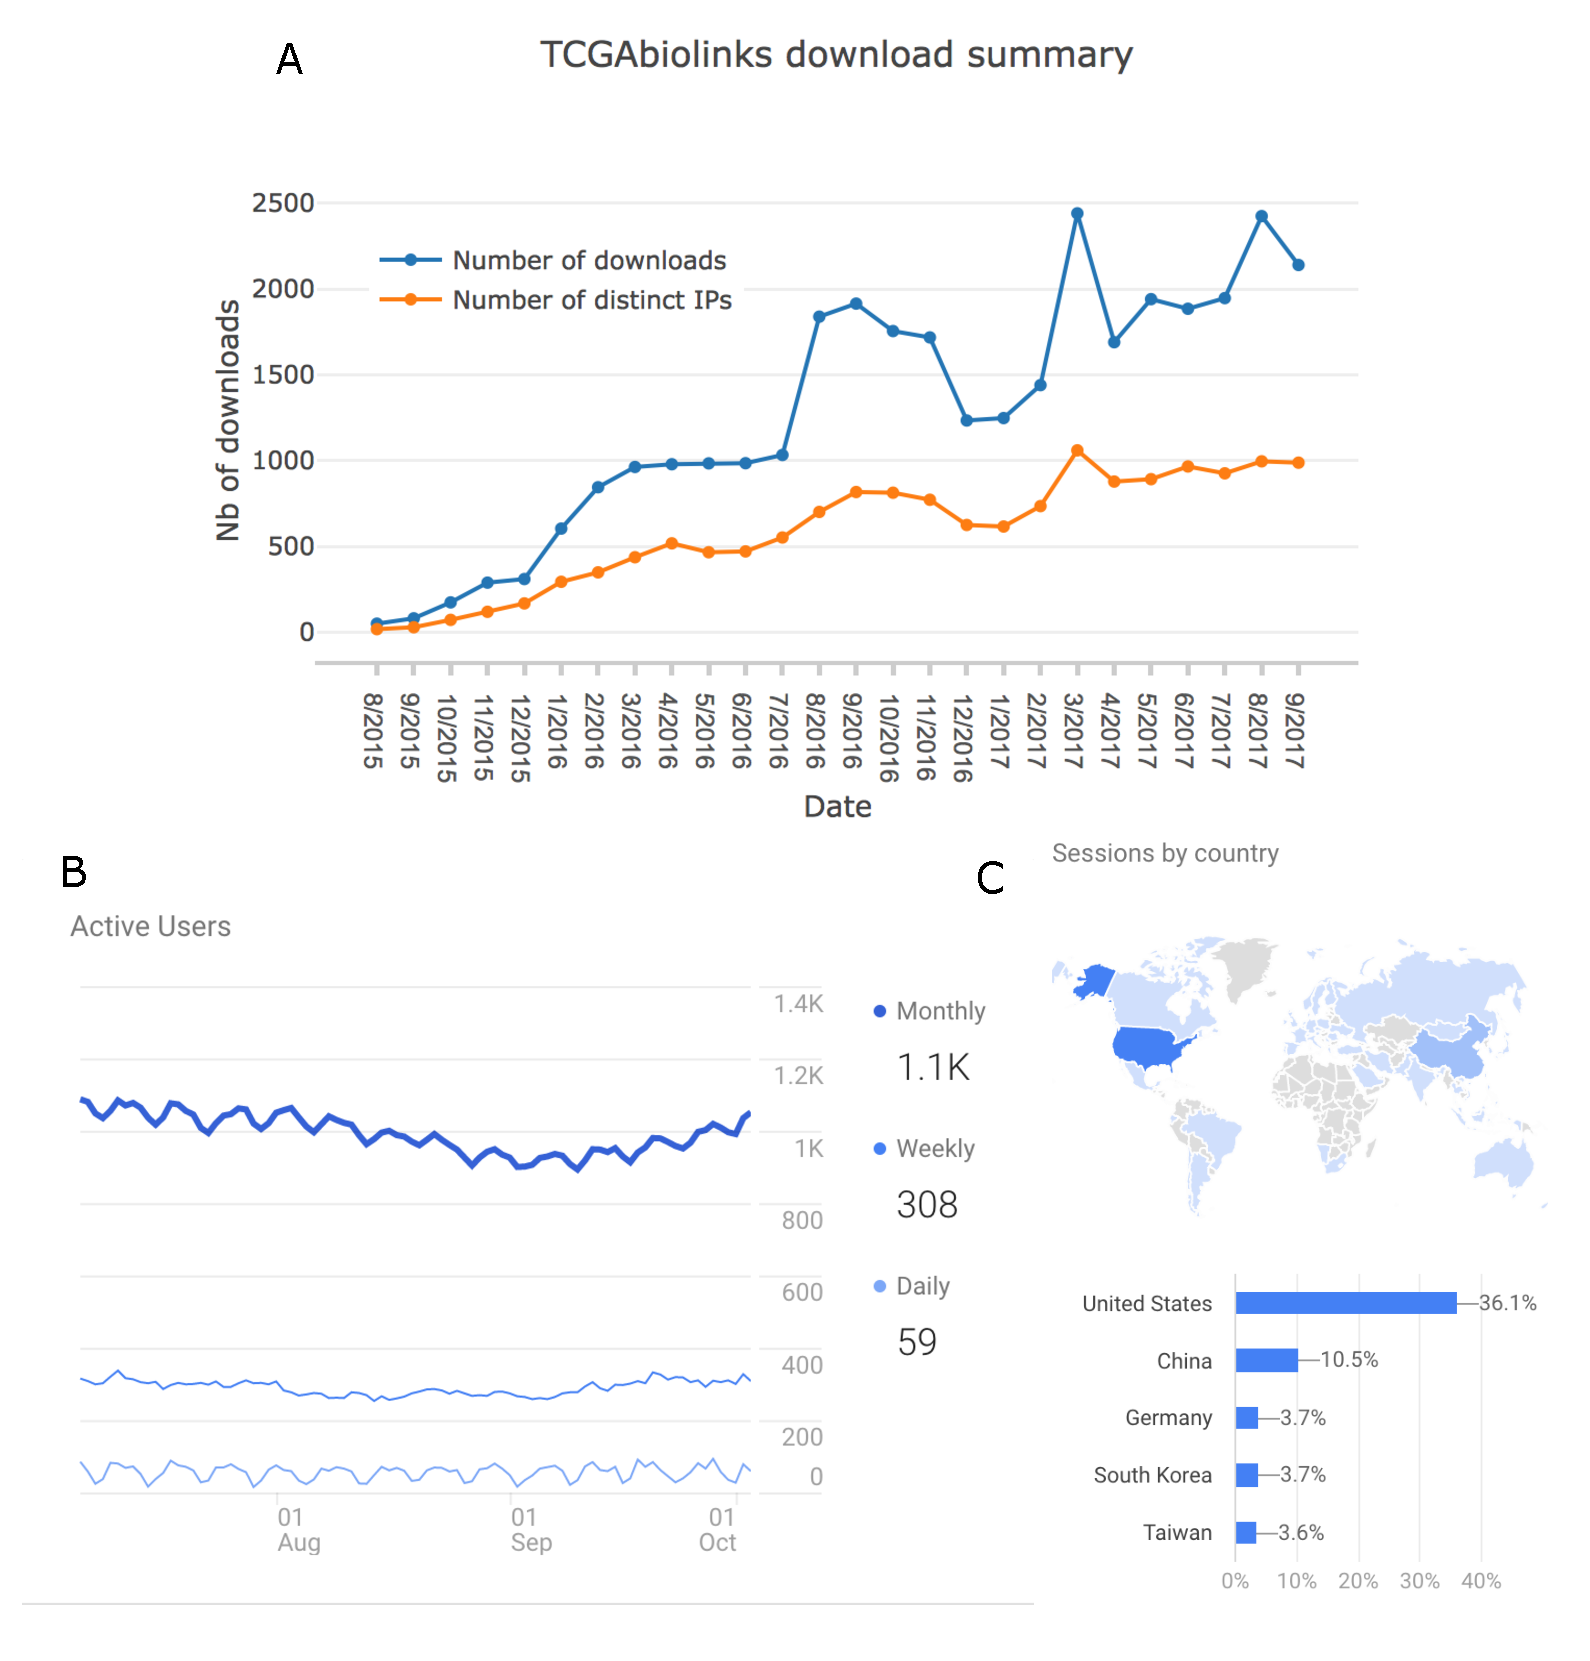
\includegraphics[width=1.0\linewidth]{images/tcgabiolinks_download.pdf}
	\caption[TCGAbiolinks download summary]{TCGAbiolinks download summary. A) Number of downloads per month. B) Number of active users. C) Percentage of sessions connect to the documentation by country.}
	\label{fig:tcgabiolinksdownload}
\end{figure*}

\subsection{Case of studies}

In this subsection, we introduce and describe the utility and application of TCGAbiolinks, we used four different TCGA cancer types
(Brain, Kidney, Breast and Colon) as examples. For each
tumor type, we describe methods to extract the different experimental
types and integrate the information into a cohesive,
biologically specific and hypothesis-driven approach.
We also describe how to generate a starburst plot \cite{noushmehr2010identification}. The
starburst plot was introduced to illustrate the results of integrating
DNA methylation and gene expression data. In
addition, we describe how TCGAbiolinks prepares data for
integration with other recently published packages, such as
ELMER \cite{yao2015inferring}, a new Bioconductor package designed to
identify candidate regulatory elements in the non-coding
regions of the genome associated with cancer. Our package
is freely available within the Bioconductor project at
\burl{http://bioconductor.org/packages/TCGAbiolinks/}.




\subsubsection*{Case study - LGG downstream analysis with gene expression}

For this case study, we used the recently available \sigla{LGG}{lower-grade glioma} data to investigate gene expression differences between the reported molecular subtypes (IDHmutant, IDHwildtype and IDHmutant codels) \cite{platforms2015comprehensive}. In particular, we used TCGAbiolinks to download 293 samples profiled using messenger RNA expression (IlluminaHiSeq RNASeqV2) with available molecular subtypes. The data was normalized using the \textit{TCGAanalyze\_Normalization} function and we applied three filters to remove features/mRNAs with low signals across samples, obtaining 4578, 4284 and 1187 mRNAs, respectively. A clustering analysis was then applied using the ConsensusClusterPlus package \cite{wilkerson2010consensusclusterplus} which identified four distinct groups of samples (EC1-EC4) (Figure \ref{fig:caseexp}A). The survival curves for each cluster were generated using \textit{TCGAanalyze\_survival} and are shown in Figure \ref{fig:caseexp}B. As expected, each cluster effectively separated IDHwildtype tumors (EC1) from IDHmutant-non-codel (EC2) and IDHmutant-codel tumors (EC3 and EC4) (Figure \ref{fig:caseexp}). Additional biological subtypes (DNA methylation subtypes) were reproduced as expected (Figure \ref{fig:caseexp}D) \cite{platforms2015comprehensive}.

\begin{figure*}
\centering
%\includegraphics[width=.9\linewidth]{figures/case3_improved.pdf}
\includegraphics[width=1.0\linewidth]{images/figure4.pdf}
\caption[Case study - LGG downstream analysis with gene expression]{Case study - Integrative (or Downstream) analysis of gene expression and clinical data from LGG disease with unsupervised clustering and crossing expression clusters with clinical and molecular information. \textbf{(A)} Heatmap of 1187 more variables genes clustered with tree $k = 4$ in EC1, EC2, EC3, EC4. \textbf{(B)} Kaplan Meier survivals plot for EC clusters. \textbf{(C and D)} Distribution of the DNA Methylation clusters and ATRX mutation within the EC clusters.}
\label{fig:caseexp}
\end{figure*}

\subsubsection*{Case study - Downstream analysis integration of gene expression and methylation data}

The DNA methylation of specific promoter CpG islands has the potential to influence gene expression.
In this case study, we used TCGAbiolinks to examine the biological relationship between DNA methylation
and gene expression in \sigla{COAD}{Colon adenocarcinoma}. Using \textit{GDCquery},\textit{GDCdownload}
and \textit{GDCprepare}, we obtained DNA methylation data (Infinium HumanMethylation450 and Infinium
HumanMethylation27 platforms) and gene expression data (IlluminaGA RNASeqV2 platform) for the same
TCGA COAD samples \cite{cancer2012comprehensive}. A supervised analysis was performed on the molecular
subtypes CIMP-Low [CIMP.L] and CIMP-High [CIMP.H].
The gene expression analysis started by the identification of outliers, followed by the normalization methods.
 Using \textit{TCGAanalyze\_DEA}, 34 DEGs ($log_2FC\geq 3.0$ and FDR $\leq 10^{-4}$) were identified.
 The result of this analysis is represented in a volcano plot (Figure \ref{fig:case_starburst}A)
 created using \textit{TCGAVisualize\_volcano}.
For the DNA methylation analysis,
using \textit{TCGAanlayze\_DMR} we identified 73 CpG-methylated probes ($\Delta\overline{\beta}\geq 0.25$ and  $FDR \leq 10^{-5}$;  (Figure \ref{fig:case_starburst}B). The DNA methylation and gene expression results were integrated as in the previous TCGA marker paper \cite{noushmehr2010identification,cancer2012comprehensive}, by generating a starburst plot (Figure \ref{fig:case_starburst}C) in which the x-axis is the $log_{10}$ of the correct P-value for DNA methylation and the y-axis is the $log_{10}$ of the correct P-value for the expression data.
The starburst plot highlights nine distinct quadrants.
To incorporate the DNA methylation difference cut-off into the  graph,
we highlighted genes that might have the potential for silencing due to epigenetic alterations.
 We highlighted five genes, EYA1, SIX2, ACSL6, OGDHL and SLC30A2, that showed a $\Delta\overline{\beta}\geq0.25$
 and a $log_2FC\geq 3.0$ between CIMP.L and CIMP.H.



\begin{figure*}
\centering
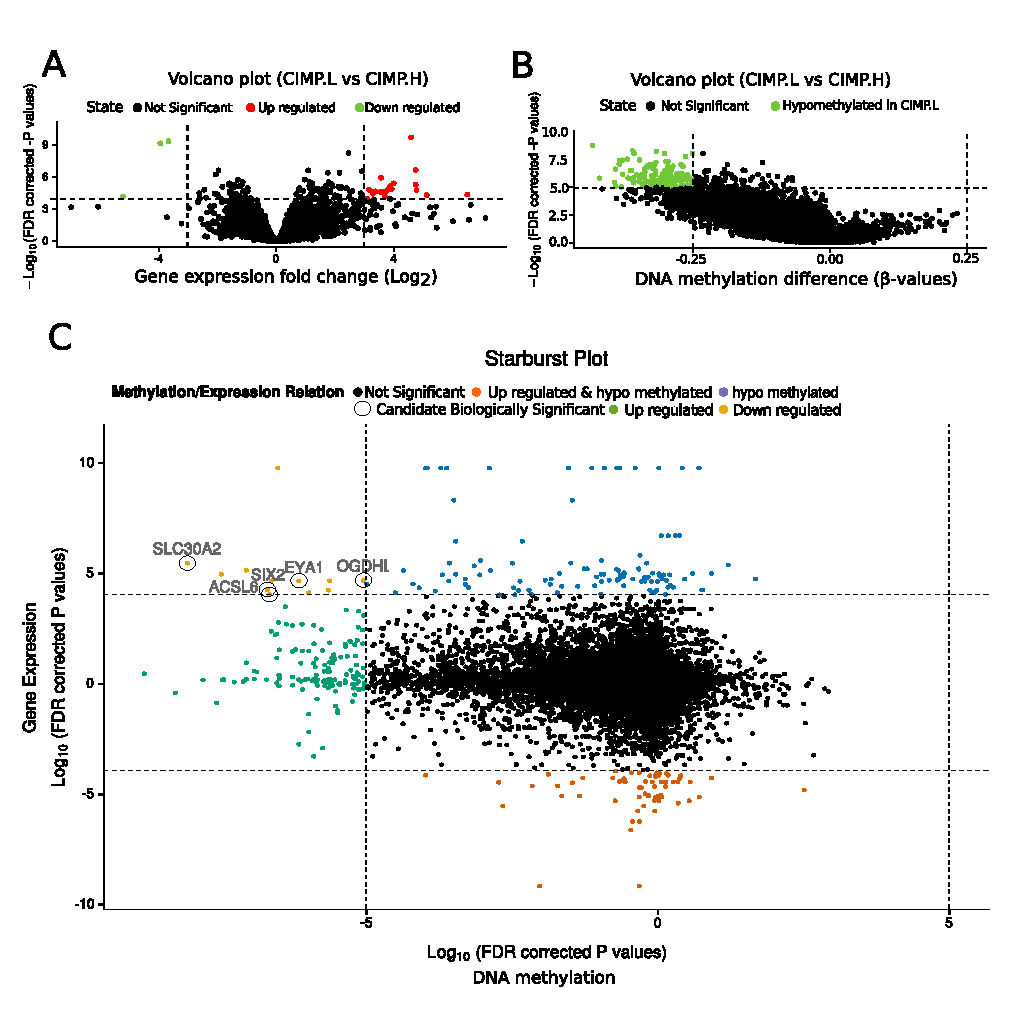
\includegraphics[width=1.0\linewidth]{images/figure5.pdf}
\caption[Case study - Integrative analysis of gene expression and DNA methylation data from COAD disease]{
Case study - Integrative analysis of gene expression and DNA methylation data from COAD disease,
comparing groups CIMP.L and CIMP.H. \textbf{(A)} Expression volcano plot: fold change of expression data versus significance.
 \textbf{(B)} DNA methylation volcano plot: difference of DNA methylation versus significance.
 \textbf{(C)} Starburst plot: DNA methylation significance versus gene expression significance.}
\label{fig:case_starburst}
\end{figure*}

\newpage
